\documentclass{article}

\usepackage[utf8]{inputenc}
\usepackage[T1]{fontenc}
\usepackage[margin=1in]{geometry}
\geometry{a4paper}
\usepackage{amsmath}
\usepackage{amssymb}
\usepackage[mathscr]{euscript}
\usepackage{tikz}

\title{Tree Enumeration}
\author{Clayton Ristow}
\date{18 June 2015}

\begin{document}
\maketitle
 
To derive the generating function for an annealed branched polymer, we need a method for counting the number of branched polymers with a specific number of nodes. We will use graph theory to count these possible arrangements of branches. However, we do not with to enumerate all graphs. We will limit ourselves to the following types our graphs.
\begin{itemize}
\item The graph will be not contain any closed loops. In other words the graphs are acyclic. 
\item The graph will be connected meaning there will be no unattached nodes. These first two qualifications define a graph called a tree. An example of a tree is shown in figure 1.
\item Each node on the graph will have no more than 3 branches protruding from it. In our model of RNA folding in on itsself, it would be highly unlikely that the RNA would fold in such a way that there would be a four way intersecion exactly. In most cases where there appears to be such an intersection, we can model it with two three way intersections sepearted by a very small branch
\end{itemize}

\begin{figure}[!h]
\centering
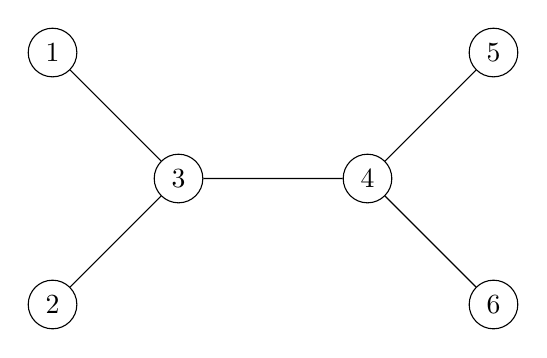
\begin{tikzpicture}
[scale=.8, every node/.style={circle,draw}]
\node (n1) at (1,7) {1};
\node (n2) at (1,3) {2};
\node (n3) at (3,5) {3};
\node (n4) at (6,5) {4};
\node (n5) at (8,7) {5};
\node (n6) at (8,3) {6};

\foreach \from/\to in {n1/n3,n2/n3,n3/n4,n4/n5,n4/n6}
	\draw (\from) -- (\to);

\end{tikzpicture}
\caption{A basic tree}
\end{figure}

\section{Polya's Enumeration Theorem}
Polya's Enumeration Theorem provides us with a very usefull tool for counting graphs. Say we have a graph G and we want to know the number of different ways to color the nodes on our graph black or white. However, we are allowed to twist rotate and flip our graph in any way as long as the connections between nodes remains constant. For example, the two decorated graphs in figure 2 are identical. 

\begin{figure}[!h]
\centering
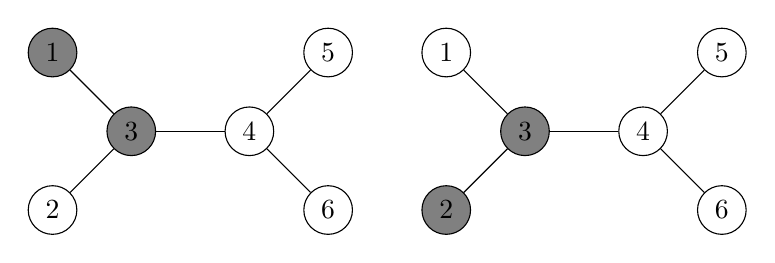
\begin{tikzpicture}
[scale=.5]
\tikzset{marked/.style={circle,draw,fill=black!50}}
\tikzset{unmarked/.style={circle,draw}}
\node [marked] (n1) at (1,7) {1};
\node [unmarked] (n2) at (1,3) {2};
\node [marked] (n3) at (3,5) {3};
\node [unmarked] (n4) at (6,5) {4};
\node [unmarked]  (n5) at (8,7) {5};
\node [unmarked] (n6) at (8,3) {6};

\node [unmarked] (n11) at (11,7) {1};
\node [marked] (n12) at (11,3) {2};
\node [marked] (n13) at (13,5) {3};
\node [unmarked] (n14) at (16,5) {4};
\node [unmarked]  (n15) at (18,7) {5};
\node [unmarked] (n16) at (18,3) {6};

\foreach \from/\to in {n1/n3,n2/n3,n3/n4,n4/n5,n4/n6,n11/n13,n12/n13,n13/n14,n14/n15,n14/n16}
	\draw (\from) -- (\to);

\end{tikzpicture}
\caption{These decorated trees are identical}
\end{figure}

We must develop some technique to deal with over counting in these situations. The answer is Polya's Enumeration Theorem. 
For every method of decorating a graph there is a decoration function 

 \begin{equation}
f(x)=f_0+f_1x+f_2x^2+f_3x^3...
\end{equation}

such that \(f_n\) is the number of ways to arrange n "somthings" on a specific node.
For every graph G there is a group of permutations \(P_G\) such that when \(P_G\) acts on the set of nodes the set of edges does not change. From this group, we may generate what is called the cycle index. the cycle index is defined as follows. Its is an elementary fact that a permutation can be written as the composition of disjoint cycles. So for each element g of the group \(P_G\) we can write what is called the cycle monomial as 

\begin{equation}
Cycle Monomial=\prod_k S_k^{j_k(g)}
\end{equation}

where k is the length of the cycle and \(j_k(g)\) is the number of cycles of length k in the element g
The cycle index \(Z_G\) is simply the sum of cycle monomials over all group elements.
 
\begin{equation}
Z_G(S_1,S_2,S_3...) \equiv \frac{1}{|P_G|}\sum_{g\in P_G} \prod_k S_k^{j_k(g)}
\end{equation}

Then finally, Polya's Enumeration Theorem says:
Let G be a graph. Let \(F(x)\) be a power series 
\begin{equation}
F(x)=F_0+F_1x+F_2x^2...
\end{equation}
where \(F_n\) is the number of ways to represent the graph with n nodes decorated. Then we may compute \(F(x)\) as
\begin{equation}
F(x)=Z_G(f(x),f(x^2),f(x^3)...)
\end{equation}
where f(x) is the decoration function and \(Z_G\) is the cycle index. 

let us use the Graph in figure 1 as an example. 
It is quite simple to find \(P_G\) for our graph in figure 1. Written in cyclic notation the permutation group is:
\begin{equation}
P_G=\{e,(12),(56),(12)(56),(1625)(34), (1526)(34),(16)(25)(34),(15)(26)(34)\}
\end{equation} 
So the cycle index is
\begin{equation}
Z_G=\frac{1}{8} (S_1^6+2S_1^4S_2^1+2S_4^1S_2^1+2S_2^3)
\end{equation}
 and because there is one way to not color in a node and one way to color in a node we can write the decoration function as
\begin{equation}
f(x)=1+x
\end{equation}
Applying Polyas Enumeration Theorem, we get 
\begin{equation}
F(x)=\frac{1}{8}((1+x)^6+2(1+x)^4(1+x^2)+2(1+x^4)(1+x^2)+2(1+x^2)^3)
\end{equation}
Which simplified becomes
\begin{equation}
F(x)=1+2x+5x^2+5x^3+5x^4+2x^5+x^6
\end{equation}
which tells us that there is one way to color in no nodes, 2 ways to color in 1 node, 5 ways to color in 2, 3, or 4 nodes, 2 ways to  color in 5 nodes, and 1 way to color in all the nodes. 

\section{Planted Trees}
We now have the tools nessessary to start enumerating some trees. We will first look at planted trees. Planted trees are a special type of tree that start with a special node that has one branch coming off of it in one direction. An example is shown in figure 3. The square node represents the special node that starts the planted tree. 
 
\begin{figure}[!h]
\centering
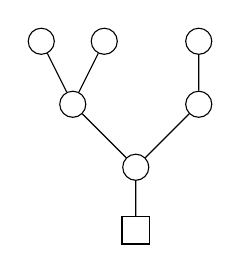
\begin{tikzpicture}
[scale=.4]
\tikzset{circ/.style={circle,draw}}
\tikzset{sq/.style={draw,minimum size=.35cm}}
\node [sq] (n1) at (5,1) {};
\node [circ] (n2) at (5,3) {};
\node [circ] (n3) at (3,5) {};
\node [circ] (n4) at (7,5) {};
\node [circ] (n5) at (2,7) {};
\node [circ] (n6) at (4,7) {};
\node [circ] (n7) at (7,7) {};

\foreach \from/\to in {n1/n2,n2/n3,n2/n4,n4/n7,n3/n5,n3/n6}
	\draw (\from) -- (\to);

\end{tikzpicture}
\caption{A planted tree}
\end{figure}

We want to find a formula to count the number of planted trees with n nodes. To do this we will find \(F(x)=F_0+F_1x+F_2x^2...\) where \(F_n\) is the number of planted trees with n nodes. We can map out the first few easily by hand (Fig. 4):

\begin{figure}[!h]
\centering
\begin{tikzpicture}
[scale=.7]
\tikzset{circ/.style={circle,draw}}
\tikzset{sq/.style={draw,minimum size=.35cm}}
\node [sq] (n1) at (1,1) {};
\node [circ] (n2) at (1,3) {};
\node at (2.5,1) {,};
\node [sq]  (n3) at (4,1) {};
\node [circ] (n4) at (4,3) {};
\node [circ] (n5) at (4,5) {};
\node at (5.5,1) {,};
\node [sq] (n6) at (7,1) {};
\node [circ] (n7) at (7,3) {};
\node [circ] (n8) at (7,5) {};
\node [circ] (n9) at (7,7) {};
\node [sq] (n10) at (9,1) {};
\node [circ] (n11) at (9,3) {};
\node [circ] (n12) at (8,5) {};
\node [circ] (n13) at (10,5) {};
\node at(11.5,1) {, . . .};

\foreach \from/\to in {n1/n2,n3/n4,n4/n5,n6/n7,n7/n8,n8/n9,n10/n11,n11/n12,n11/n13}
	\draw (\from) -- (\to);
\end{tikzpicture}
\caption{All of the planted trees with 2, 3, of 4 nodes}
\end{figure}

However, to enumerate for larger n, we can find a functional equation for \(F(x)\) by decorating the trees with other rooted trees. By definition the tree must start with a square node connected to a normal circular node as shown in figure 5. 

\begin{figure}[!h]
\centering
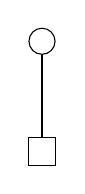
\begin{tikzpicture}
[scale=.7]
\tikzset{circ/.style={circle,draw}}
\tikzset{sq/.style={draw,minimum size=.35cm}}
\node [sq] (n1) at (1,1) {};
\node [circ] (n2) at (1,3) {};

\foreach \from/\to in {n1/n2}
	\draw (\from) -- (\to);
\end{tikzpicture}
\caption{All planted trees start this way}
\end{figure}

This starting graph has two nodes already so whatever is attached to the top node will already have two nodes attached to it. So we start the functional equation as:
\begin{equation}
F(x)=x^2(\text{number of ways to attach planted trees to the top node})
\end{equation}

There are 3 ways to attach planted trees to the top node given our framework (Fig. 6). Our options are attach nothing to the top node, attach 1 planted tree to the top node or attach 2 planted trees to the top node.

\begin{figure}[!h]
\centering
\begin{tikzpicture}
[scale=.7]
\tikzset{circ/.style={circle,draw}}
\tikzset{sq/.style={draw,minimum size=.35cm}}
\node [sq] (n1) at (1,1) {};
\node [circ] (n2) at (1,3) {};
\node at (2.5,1) {,};
\node [sq]  (n3) at (4,1) {};
\node [circ] (n4) at (4,3) {};
\node (n5) at (4,5) {};
\node at (5.5,1) {,};
\node [sq] (n6) at (7,1) {};
\node [circ] (n7) at (7,3) {};
\node (n8) at (6,5) {};
\node (n9) at (8,5) {};

\foreach \from/\to in {n4/n5,n7/n8,n7/n9}
	\draw [dashed] (\from) -- (\to);
\foreach \from/\to in {n1/n2,n3/n4,n6/n7}
	\draw (\from) -- (\to);
\end{tikzpicture}
\caption{3 ways to decorate the two node starter graph: 0, 1, or 2 planted trees}
\end{figure}

Now let us enumerate each way of decorating the graph.There is clearly only one way to add no planted trees on the top node so this decoration contributes 1. Next, the number of ways to add one planted trees is simply the number of planted trees there are to add, which is represented by F(x). However by adding the square node on top of the circular node we are over counting the nodes by 1 so we must divide by x to lower the node count by 1. Thus adding one planted tree contributes \(\frac{F(x)}{x}\). Adding two trees becomes a little tricky. Clearly the branched graphs can flip sides with out chaning the enitre graph so we will be over counting the total number of graphs. We can use Polya's Enumeration Theorem to deal with this overcounting. Flipping two things results in a symmetry group isomorphic to the symmetric group of order 2. Our decoration function is the number of planted trees so our decoration function is \(F(x)\). Finally, since we are adding two square nodes on top of the top node we must divide by \(x^2\) to adjust for over counting these nodes. So the contribution from adding 2 planted trees is \(\frac{1}{x^2}(Z_{S_2}(F(x),F(x^2),F(x^3)...))\). Combining all of these contributions and plugging into Eq. 11 we get:
\begin{equation}
F(x)=x^2(1+\frac{F(x)}{x}+\frac{1}{x^2}(Z_{S_2}(F(x),F(x^2),F(x^3)...)))
\end{equation}
 
The symmetric group of order 2 written in cyclic notation is 
\begin{equation}
S_2=\{e,(12)\}
\end{equation}
Clearly then its cycle index is 
\begin{equation}
Z_{S_2}=\frac{1}{2}(S_1^2+S_2^1)
\end{equation}
Then plugging this cycle index into equation 12 we get:
\begin{equation}
F(x)=x^2(1+\frac{F(x)}{x}+\frac{1}{2x^2}(F^2(x)+F(x^2))
\end{equation}
And then from simplyfing we arrive at our functional equation:
\begin{equation}
F(x)=x^2+ xF(x)+\frac{1}{2}F^2(x)+\frac{1}{2}F(x^2)
\end{equation}

We can find a recursive formula for \(F_n\) fairly easily by remembering the \(F(x)\) is a power series written as 
\begin{equation}
F(x)=\sum_{n=0}^\infty F_nx^n
\end{equation}
Then we can plug this power series into the functional equation to get
\begin{equation}
\sum_{n=0}^\infty F_nx^n=x^2+\sum_{n=0}^\infty F_nx^{n+1}+\frac{1}{2}\sum_{n=0}^\infty \sum_{m=0}^\infty F_n F_mx^{m+n}+\frac{1}{2}\sum_{n=0}^\infty F_nx^2n
\end{equation}
We can equate like powers of x to each other so if n is greater than 2 we get:
\begin{equation}
F_nx^n=
\begin{cases}
F_{n-1}x^n+\frac{1}{2}\sum_{i=0}^nF_iF_{n-i}x^n+\frac{1}{2}F_{\frac{n}{2}}x^n &\text{if } x \text{ is even} \\
F_{n-1}x^n+\frac{1}{2}\sum_{i=0}^nF_iF_{n-i}x^n & \text{if }x \text{ is odd} 
\end{cases}
\end{equation}
then canceling the \(x^n\) and expanding we get:
\begin{equation}
F_n=
\begin{cases}
F_{n-1}+ \frac{1}{2}(F_0F_n+F_1F_{n-1}+...+F_{n-1}F_1+F_nF_0)+\frac{1}{2}F_{\frac{n}{2}} &\text{if } x \text{ is even} \\
F_{n-1}+\frac{1}{2} (F_0F_n+F_1F_{n-1}+...+F_{n-1}F_1+F_nF_0) & \text{if }x \text{ is odd} 
\end{cases}
\end{equation}
which can be consolidated as
\begin{equation}
F_n=
\begin{cases}
F_{n-1}+ \frac{1}{2}(2F_0F_n+2F_1F_{n-1}+...+F_n^2)+\frac{1}{2}F_{\frac{n}{2}} &\text{if } x \text{ is even} \\
F_{n-1}+\frac{1}{2} (2F_0F_n+2F_1F_{n-1}+...+2F_{\frac{n}{2}-1}F_{\frac{n}{2}+1}) & \text{if }x \text{ is odd} 
\end{cases}
\end{equation}
and then if we recall that \(F_0=F_1=0\) we can write a final recurrance relation:
\begin{equation}
F_n=
\begin{cases}
F_{n-1}+\sum_{i=2}^{\frac{n}{2}-1}F_iF_{n-i}+\frac{1}{2}(F_{\frac{n}{2}}+F_{\frac{n}{2}}^2) &\text{if } x \text{ is even} \\
F_{n-1}+\sum_{i=2}^{\frac{n-1}{2}}F_iF_{n-i} & \text{if }x \text{ is odd} 
\end{cases}
\end{equation}
with \(F_2=1\)

\section{Rooted Trees}
The next step toward enumerating general trees is to enumerate rooted trees. Rooted trees are trees that start with a root node (represented by a square). Unlike planted trees, rooted trees can have more than one branch attached to it. An example of a rooted tree is shown in figure 7.

\begin{figure}
\centering
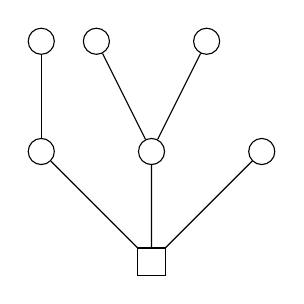
\begin{tikzpicture}
[scale=.7]
\tikzset{circ/.style={circle,draw}}
\tikzset{sq/.style={draw,minimum size=.35cm}}
\node [sq] (n1) at (5,1) {};
\node [circ] (n2) at (3,3) {};
\node [circ] (n3) at (5,3) {};
\node [circ] (n4) at (7,3) {};
\node [circ] (n5) at (3,5) {};
\node [circ] (n6) at (4,5) {};
\node [circ] (n7) at (6,5) {};

\foreach \from/\to in {n1/n2,n1/n3,n1/n4,n2/n5,n3/n6,n3/n7}
	\draw (\from) -- (\to);

\end{tikzpicture}
\caption{A rooted tree}
\end{figure}

We can expand upon our knowledge of planted trees to count rooted trees. Clearly, we can construct rooted trees by decorating the root node with 0, 1, 2 or 3 planted trees (Fig. 8). Let \(R(x)\) be a power series with coefficients \(R_n\) being the number on rooted trees with n nodes. Using Polya's Enumeration Theorem, we can get a functional equation for \(R(x)\) in terms of \(F(x)\) by decorating the root node with 0, 1, 2, or 3 planted trees. 

\begin{figure}[h]
\centering
\begin{tikzpicture}
[scale=.7]
\tikzset{circ/.style={circle,draw}}
\tikzset{sq/.style={draw,minimum size=.35cm}}
\node [sq] (n1) at (1,1) {};
\node at (2.5,1) {,};
\node [sq]  (n2) at (4,1) {};
\node (n3) at (4,3) {};
\node at (5.5,1) {,};
\node [sq] (n4) at (7,1) {};
\node (n5) at (6,3) {};
\node (n6) at (8,3) {};
\node at (9,1) {,};
\node [sq] (n7) at (11,1) {};
\node (n8) at (9,3) {};
\node (n9) at (11,3) {};
\node (n10) at (13,3) {};

\foreach \from/\to in {n2/n3,n4/n5,n4/n6,n7/n8,n7/n9,n7/n10}
	\draw [dashed] (\from) -- (\to);
\end{tikzpicture}
\caption{4 ways to decorate the root node: 0, 1, 2  or 3 planted trees}
\end{figure}

The Functional equation we get from constructing rooted trees this way is
\begin{equation}
R(x)=x\Big(1+\frac{F(x)}{x}+\frac{1}{x^2}Z_{S_2}(F(x),F(x^2)) +\frac{1}{x^3}Z_{S_3}(F(x),F(x^2),F(x^3))\Big)
\end{equation}

	Let us break Eq. 23 down term by term. The x out front comes fron counting the root node. The 4 terms inside the parenthesis come from the 4 ways to decorate with planted trees. The 1 comes from decorating with 0 nodes. Clearly there is only one way to do this. The second term, \(\frac{F(x)}{x}\) comes from adding one planted tree. The number of ways to add one planted tree is simply the number of planted trees represented by \(F(x)\). The \(\frac{1}{x}\) comes from the fact that when we add the base node from the planted tree on top of the root node we over count the number of nodes by one. The third term in the parenthesis comes from adding 2 planted trees. The fact that we can swap the positions of the two added trees and we get the same resulting graph gives us a permuataion group for the added trees of \(S_2\) so we enumerate these graphs using Polya's Enumeration Theorem. The \(\frac{1}{x^2}\) comes from over countingn the base nodes added on top of the root nodes. Finally, the last term comes from adding 3 trees. Again we may swap any of the added trees with any of the other trees resulting in a permutation group \(S_3\). Again we use polya's enumeration theorem and divide by \(x^3\) to adjust for over counting the base nodes. 
	
	We can simplify this equation immediately. If we recall the Functional equation for F(x) in the form it was in in Eq. 12, we can see the first 3 terms in equation 23 are equal to \(\frac{F(x)}{x^2}\). We can then make the following substitution to get
\begin{equation}
R(x)=x\Big(\frac{F(x)}{x^2} +\frac{1}{x^3}Z_{S_3}(F(x),F(x^2),F(x^3))\Big)
\end{equation}

Now we must find the cycle index for \(S_3\). Write \(S_3\) in cyclic notation as:
\begin{equation}
S_3=\{e,(12),(13),(23),(123),(321)\}
\end{equation}
So we can easily compute its cycle index
\begin{equation}
Z_{S_3}=\frac{1}{6}(S_1^3+3S_2^1S_1^1+2S_3^1)
\end{equation}
Then we can rewrite Eq. 24 with this cycle index as
\begin{equation}
R(x)=x\Big(\frac{F(x)}{x^2} +\frac{1}{6x^3}(F^3(x)+3F(x^2)F(x)+2F(x^3))\Big)
\end{equation}
And finally with a little simplification we get:
\begin{equation}
R(x)=\frac{F(x)}{x} +\frac{F^3(x)}{6x^3}+\frac{F(x^2)F(x)}{2x^2}+\frac{F(x^3)}{3x^2}
\end{equation}

 Now let us substitute the respective power series for \(R(x)\) and \(F(x)\) and derive a relationship between the coefficients.
\begin{equation}
\sum_{n=0}^\infty R_nx^n= \frac{1}{x}\sum_{n=0}^\infty F_nx^n +\frac{1}{6x^2}\Big(\sum_{n=0}^\infty F_nx^n \Big)^3+\frac{1}{2x^2}\Big(\sum_{n=0}^\infty F_nx^{2n} \Big)\Big(\sum_{m=0}^\infty F_mx^m \Big) +\frac{1}{3x^2}\sum_{n=0}^\infty F_nx^{3n}
\end{equation}
With a little simplification we get\begin{equation}
\sum_{n=0}^\infty R_nx^n= \sum_{n=0}^\infty F_nx^{n-1} +\frac{1}{6}\sum_{i=0}^\infty \sum_{j=0}^\infty \sum_{k=0}^\infty  F_iF_jF_kx^{i+j+k-2}+\frac{1}{2}\sum_{i=0}^\infty \sum_{j=0}^\infty F_iF_jx^{i+2J-2} +\frac{1}{3}\sum_{n=0}^\infty F_nx^{3n-2}
\end{equation}
Then we equate the like powers of x:
\begin{equation}
 R_nx^n=  F_{n+1}x^n +\frac{1}{6}\sum_{i=0}^{n+2} \sum_{j=0}^{n+2-i} F_iF_jF_{n+2-i-j}x^n+\frac{1}{2}\sum_{i=0}^{n+2}  F_iF_{\frac{n-i}{2}+1}x^n+\frac{1}{3} F_{\frac{n+2}{3}}x^n
\end{equation}
Then we cancel the \(x^n\)s and get our final formula for rooted trees.
\begin{equation}
 R_n=  F_{n+1} +\frac{1}{6}\sum_{i=0}^{n+2} \sum_{j=0}^{n+2-i} F_iF_jF_{n+2-i-j}+\frac{1}{2}\sum_{i=0}^{n+2}  F_iF_{\frac{n-i}{2}+1}+\frac{1}{3} F_{\frac{n+2}{3}} \quad \text{Where } F_q=0 \text{ if } q \notin \mathbb{Z}
\end{equation}
\end{document}
